\newcommand{\LYCORIS}{{\textsc{Lycoris}}\xspace}
\newcommand{\DESYII}{{\mbox{DESY II}}\xspace}
\newcommand{\DIITBF}{{\DESYII Test Beam Facility}\xspace}
\newcommand{\SID}{{SiD}\xspace}
\newcommand{\KPIX}{{KPiX}\xspace}


\section{\KPIX Silicon Tracking}
Most recent update: 2020-05-1135 \\
Contact person: Marty Breidenbach (email: mib@slac.stanford.edu)\\
Contact person: Marcel Stanitzki (email: marcel.stanitzki@desy.de)\\
Contact person: Mengqing Wu (email: mengqing.wu@desy.de)\\




\subsection{Introduction}
The baseline design of the \SID Tracker as presented in the ILC TDR~\cite{Behnke:2013lya} is based on an all-silicon approach.
The main tracker technology of choice is silicon strip sensors arrayed in five nested cylinders in the central
region and four disks following a conical surface with an angle of 5~degrees with respect to the normal to the 
beam line in each of the end regions. The geometry of the end-caps minimizes the material budget to enhance 
forward tracking. The basic building block is a module consisting of a single-sided silicon sensor, two \KPIX readout ASICS and a small Kapton-flex cable
for power delivery and signal distribution.
The sensors have a size of approximately 10 $\times$ 10 cm$^2$, a strip pitch of \SI{25}{\micro\meter} and a readout pitch of \SI{50}{\micro\meter}.
The end-caps utilizes two modules back-to-back for small angle stereo measurements. 
Each sensor is read out by two \KPIX ASICS and connected to the DAQ and the power-supply system using a small Kapton-flex cable. This hybrid-less design 
further reduces the material budget leading two a very light-weight tracking system. A drawing of a Tracker module is shown in 
Figure~\ref{fig:SiliconTrackin:KPiX:module}.


\begin{figure}
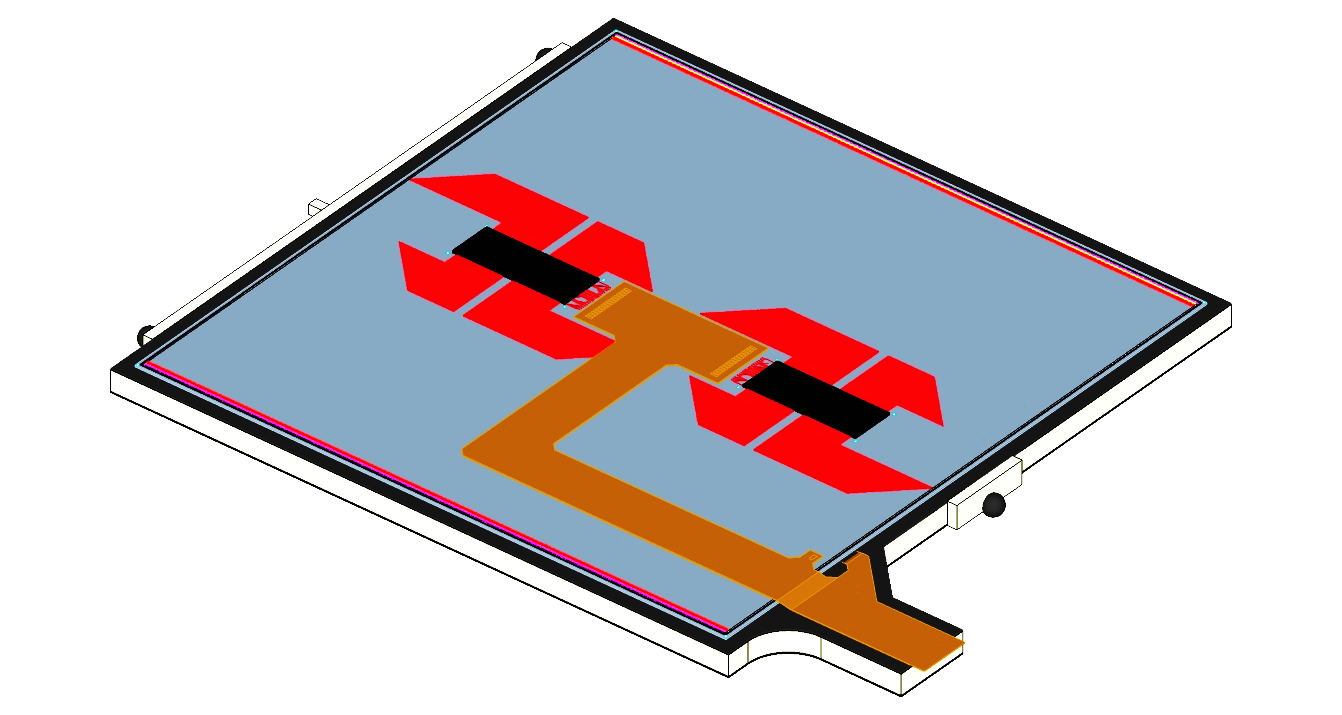
\includegraphics[width=0.49\textwidth]{Tracker/KPIX/Tracker_Module_SiD_Drawing.png}
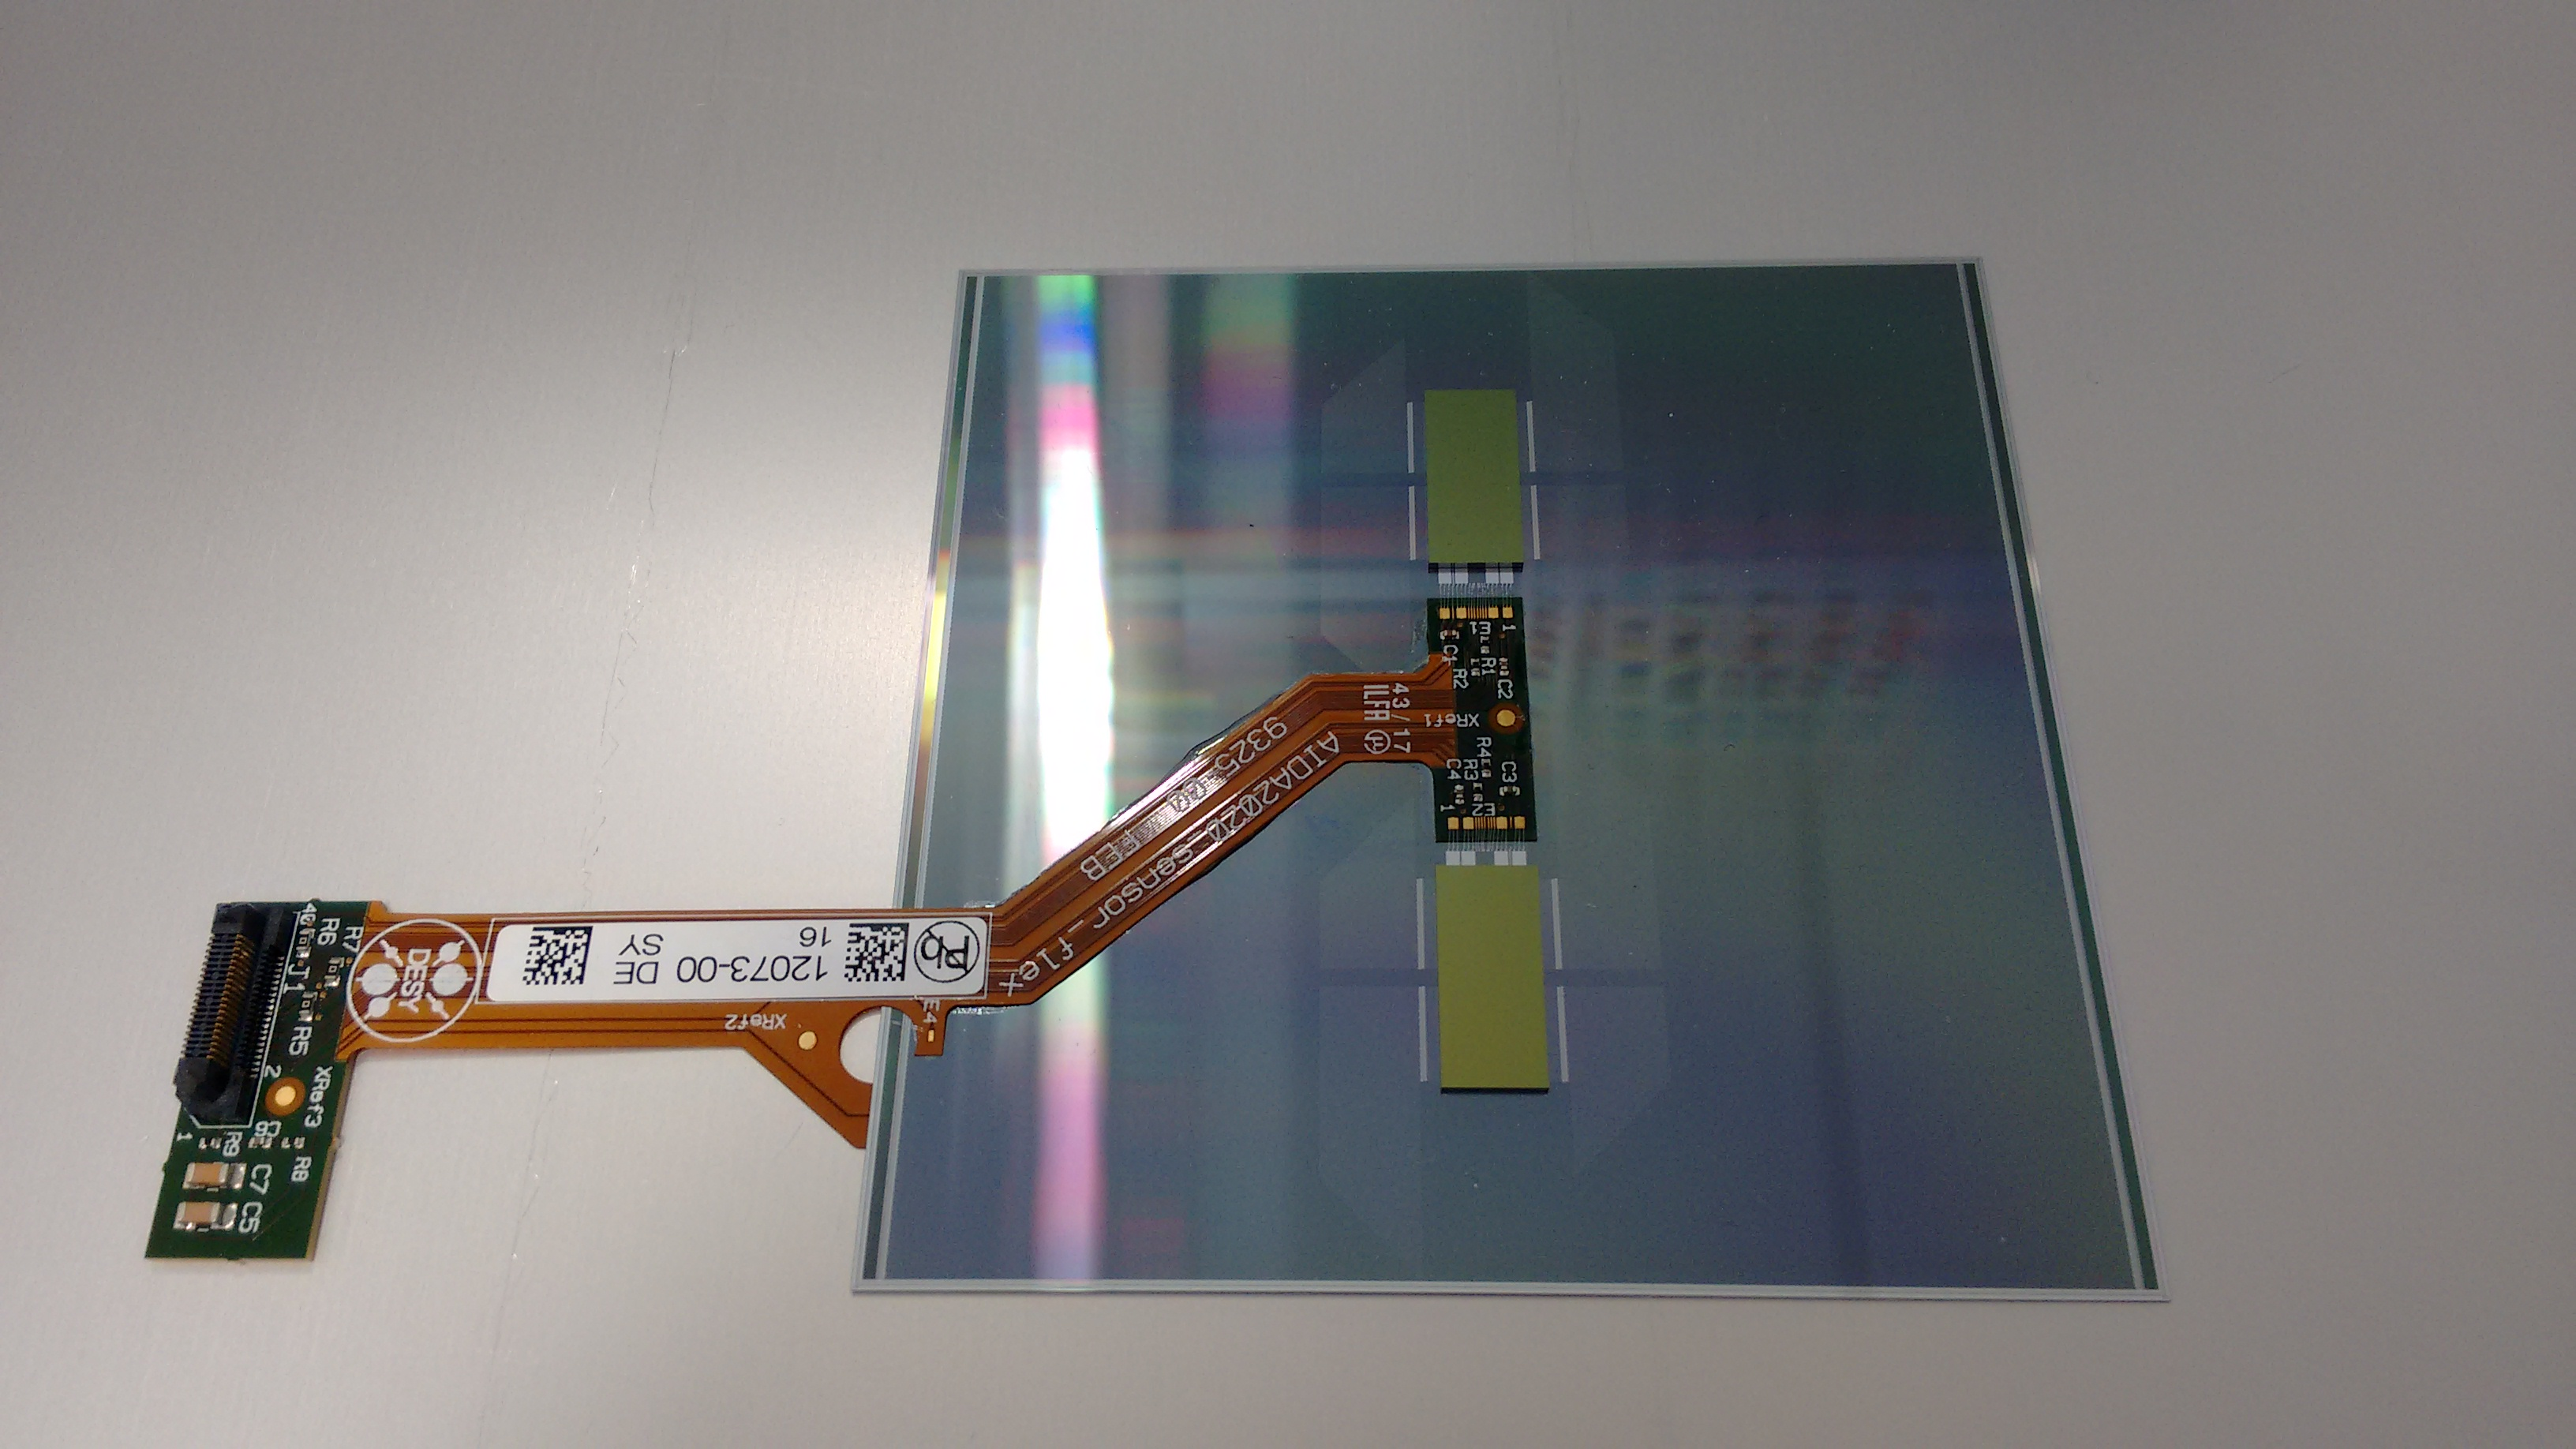
\includegraphics[width=0.49\textwidth]{Tracker/KPIX/Tracker_Module_SiD_Photo.jpg}
\caption{This \SID Tracker Module as foreseen for the baseline \SID Tracker\cite{Behnke:2013lya} with the two \KPIX ASICS and the Kapton-Flex cable 
and a first prototype sensor fully completely assembled at DESY}
\label{fig:SiliconTrackin:KPiX:module}
\end{figure}

The \KPIX ASIC~\cite{6551433}is a 1024 channel ``System on a Chip'' intended for bump bonding 
to large area silicon sensors, enabling low multiple scattering silicon-strip 
tracking and high density Particle Flow calorimetry for \SID at the ILC. 
Each channel consists of a dynamically switchable gain charge amplifier; 
shaping; threshold discrimination; and four sample and hold 
capacitors and four timing registers. The chip permits four  separate measurements of 
amplitude and time of threshold crossing during each train, and amplitude 
digitization and readout during the inter-train period. The dynamic range is from 
sub minimum ionizing particle (MIP) (in \SI{320}{\micro\meter} silicon) to more 
than 2000 MIP. \KPIX also has a calibration system for each channel, servos for 
leakage compensation, ``DC'' reset for asynchronous operation for testing with 
cosmic rays, and polarity inversion for use with GEMs and similar detectors. The 
noise floor is about \SI{0.15}{fC} ($\simeq$ 1000 electrons), and the maximum 
signal is \SI{10}{pC} (utilizing the dynamic range switching). The full dynamic 
range corresponds to 17 bits. \KPIX was manufactured using a \SI{250}{\nano\meter} process at TSMC.

\subsection{Recent Milestones}
ILC related R\&D in the US has been largely unfunded and small efforts are being kept alive. The \KPIX R\&D is such an example of necessary work for \SID.
In the last three years, the R\&D for \KPIX Silicon Tracker has been used to design and build a large-area silicon-strip 
telescope -- called \LYCORIS -- for the \DIITBF~\cite{desytb2018} as part of the Horizon2020-funded AIDA2020~\cite{AIDA2020} project.
\LYCORIS did require both the coverage of a large area (10 $\times$ \SI{10}{\centi\meter}

Based on the experiences with the first set of sensors, the second generation of sensors was produced by Hamamatsu 
using Au pads for the \KPIX bump-bonds and with a thicker oxide-layer. This was necessary, because the first generation Tracker sensor could not be 
wire-bonded to its (very thin) cable, which was unexpected. It was discovered, that the sensor oxide layer was not strong enough 
to allow wire bonding without damaging the sensor itself.

These changes have proven successful and these sensors were successfully bump-bonded to two \KPIX ASICS and wire-bonded to their Kapton-flex pigtail 
(See Figure~\ref{fig:SiliconTrackin:KPiX:module}. 

The \LYCORIS telescope has been succesfully assembled and 



\subsection{Engineering Challenges}
At this time, \KPIX is seen as the baseline readout system for both the \SID tracker and electromagnetic calorimeter. 

The \LYCORIS telescope has demonstrated that the hybrid-less approach works well, the issues both with wire-bonding and 
bump-boding have been addressed and the modules can be made with a high yield - albeit this is based on small statistics.

There remain however some noise issues with the current \KPIX design, particular in the so-called high-gain mode, 
which is important for the tracker. This is currently under detailed study and the results will inform a possible 
next-generation \KPIX. Another concern is that the current design of \KPIX has dead time after a pixel 
has accepted a trigger. Only the triggered pixel is affected; all the other 
pixels are available for signals. This dead time is different from the usual 
notion of data acquisition dead time where the entire detector is unavailable, 
but the correction to the luminosity integral is easy. Finally, the buffer 
requirement (four in the current version of \KPIX) has being re-evaluated in \SID  
simulations using the latest beam background estimates. The conclusions are, that particularly for the end-caps a move to 8 or more buffers is beneficial.
A possible new architecture for \KPIX is in early stages of  evaluation.


\subsection{Future Plans}
\LYCORIS is now going to be used at the \DIITBF and is made avaialble to all users. This will yield essential long-term operational experience and 
advance the experience with the hybrid-less modules.  

For \KPIX a new architecture with little (or no) deadtime will be evaluated. A decision will be made to develop this new architecture or incrementally 
improve the existing design. At the same time, \SID will discuss, whether moving to a fully monolithic tracker sensor is beneficial given the past technological 
developments and the timescales involved.

	
	
Assuming positive developments with Japan are announced soon, we expect the financial support to improve globally. It should be noted that
an important effect of the withdrawal of support is the slow decay of expertise, with many collaborators having to work on other projects. We expect, that 
a positive statement will lead to resurgence of interest in this technology./

	
\subsection{References}

\begin{itemize}
\item \fullcite{lycoris-D15.2}
\item \fullcite{Kraemer:2018qzh}
\item \fullcite{Kraemer:2019xku}
\item \fullcite{Wu:2020jdk}
\end{itemize}
